\documentclass[11pt]{article}

\usepackage{../macros}
\usepackage{style}

\title{Notes on Varieties of Semiring Solvers}

\author{Amaury Mazoyer}

\begin{document}

\maketitle

\tableofcontents

\newpage

\section{Preliminaries}

\begin{figure*}[!h]
  \centering
  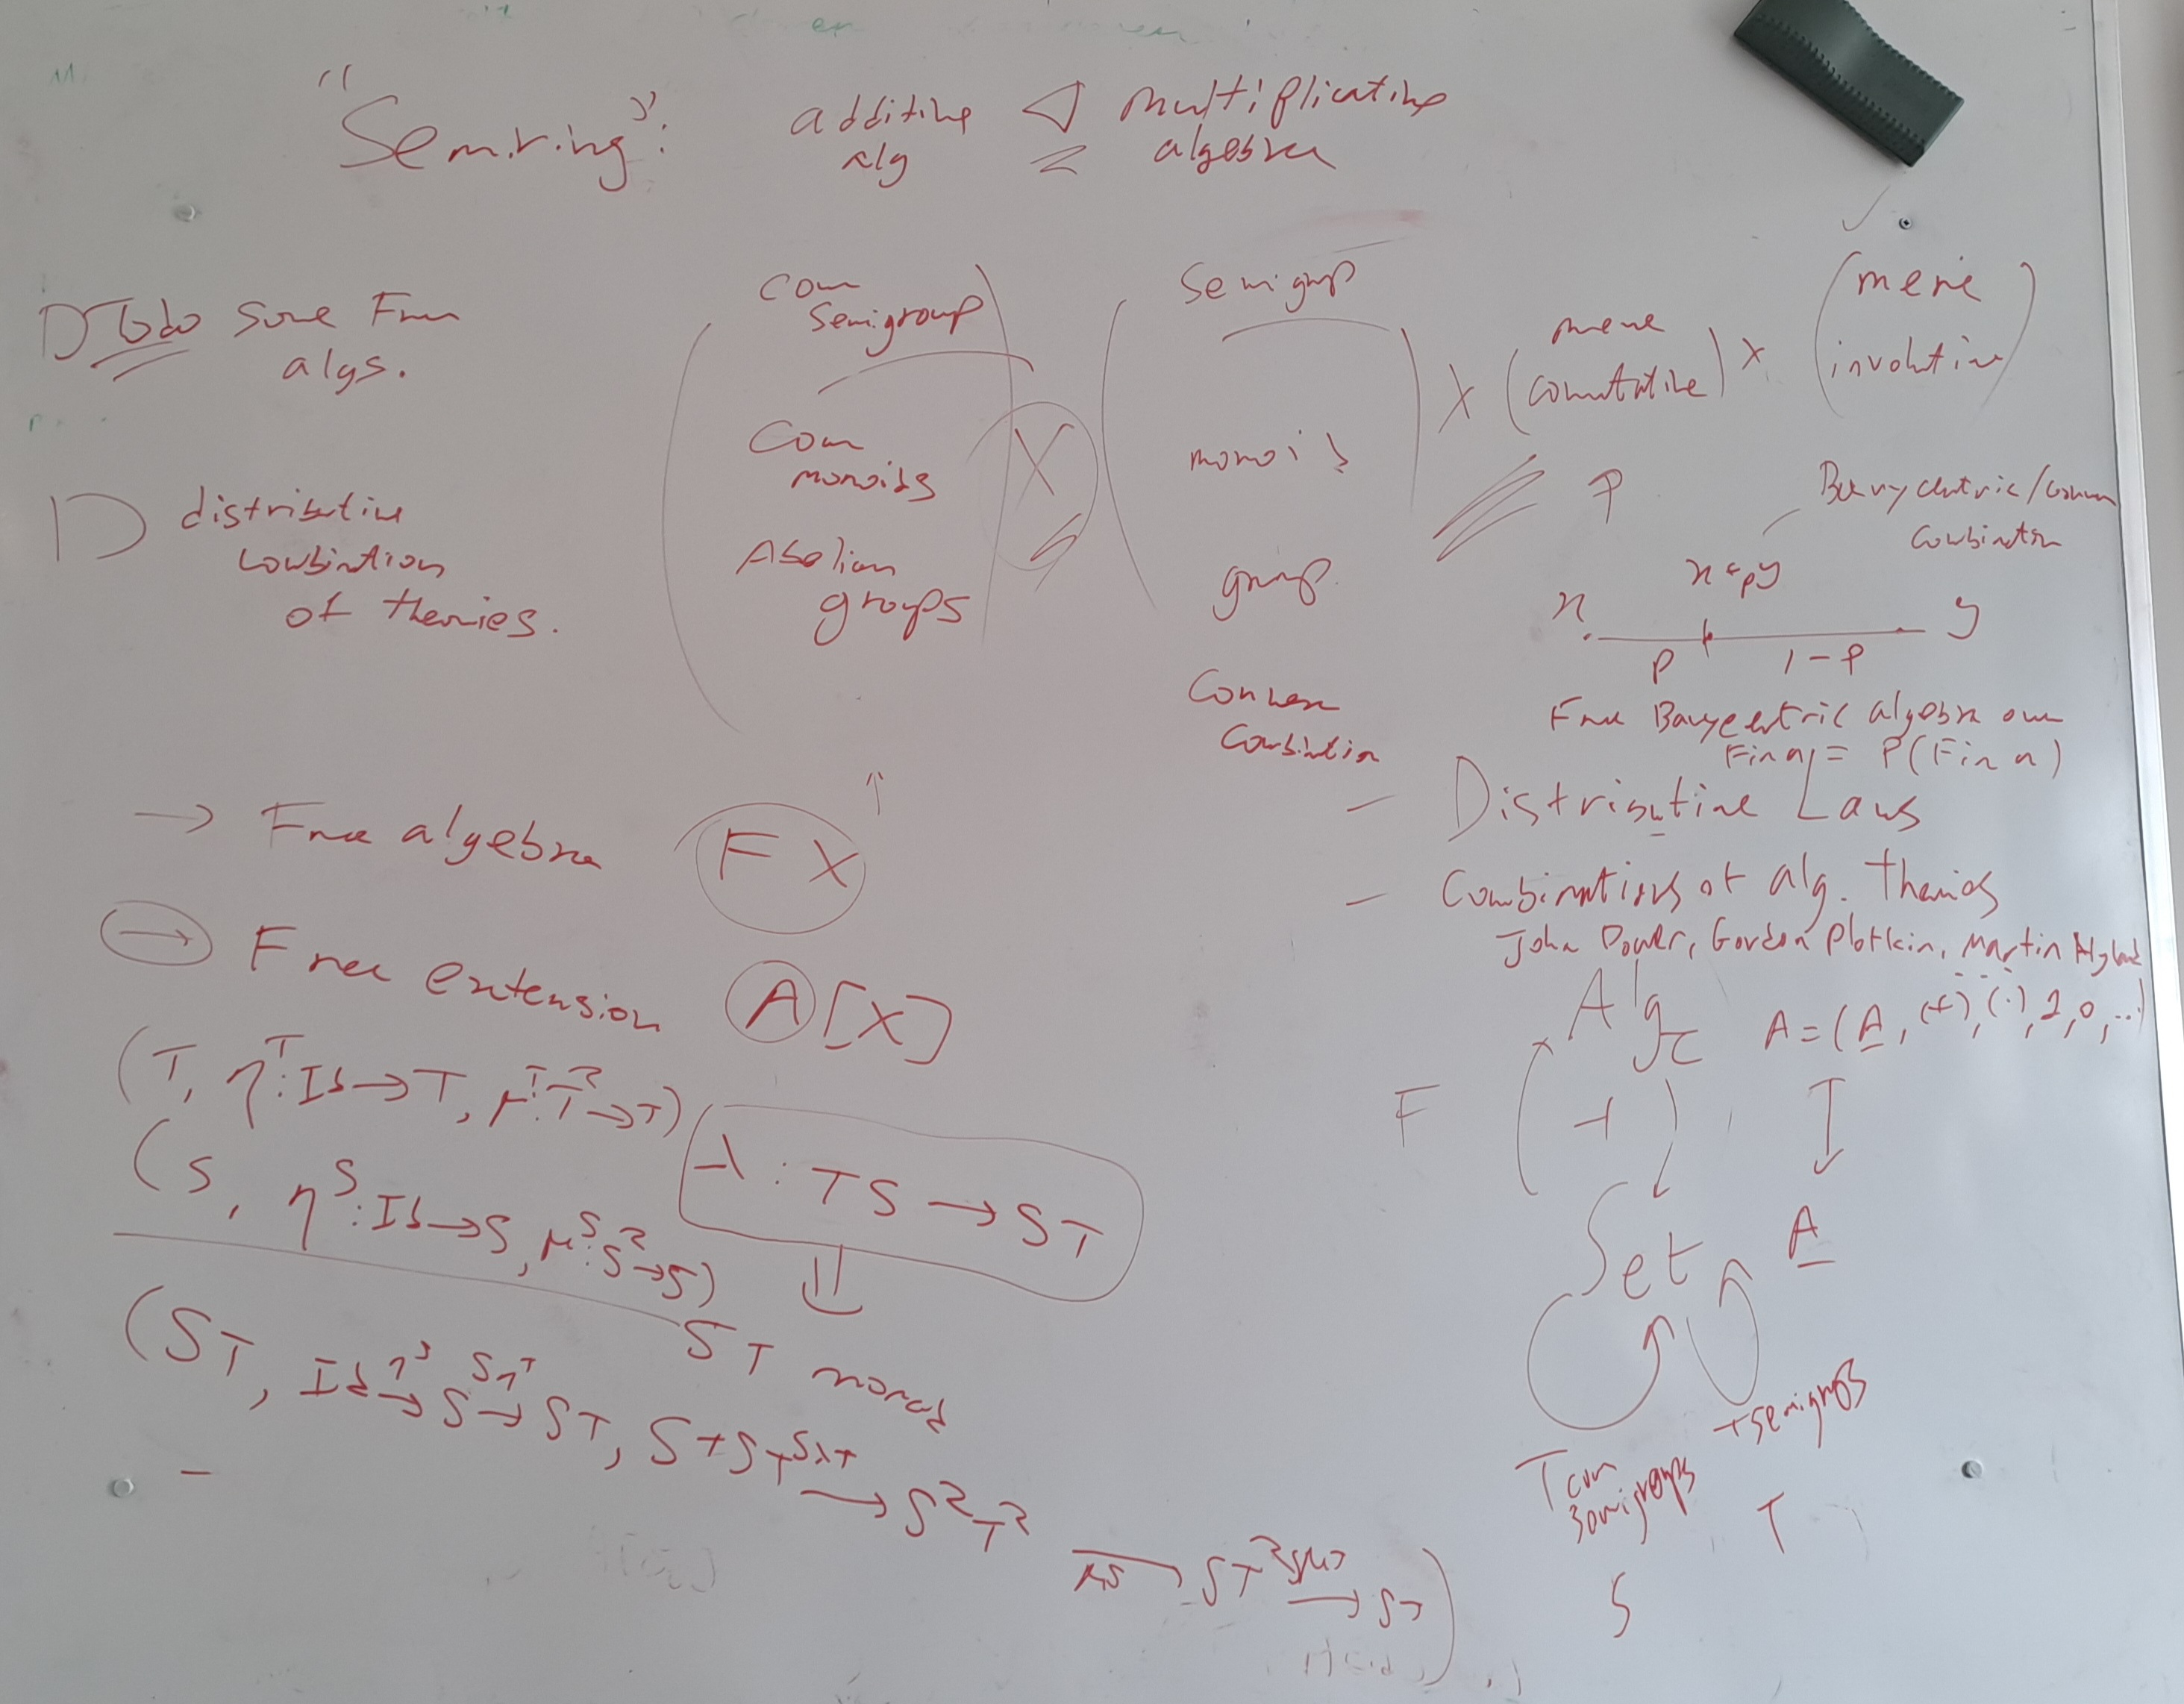
\includegraphics[width=\textwidth]{images/blackboard_start.jpg}
  \caption{Blackboard at the start of the internship.}
\end{figure*}

For convenience, we recall some definitions we'll be using.

\subsection{Algebraic Structures}

\begin{definition}[Semigroup]
  A \emph{semigroup} is a set $S$ equipped with an associative binary operation $\cdot : S \times S \to S$ such that for all $a, b, c \in S$:
  \begin{itemize}
    \item $a \cdot (b \cdot c) = (a \cdot b) \cdot c$ (associativity)
  \end{itemize}
\end{definition}

\begin{definition}[Monoid]
  A \emph{monoid} is a set $M$ equipped with an associative binary operation $\cdot : M \times M \to M$ and an identity element $e \in M$ such that for all $a, b, c \in M$:
  \begin{itemize}
    \item $a \cdot (b \cdot c) = (a \cdot b) \cdot c$ (associativity)
    \item $e \cdot a = a \cdot e = a$ (identity element)
  \end{itemize}
\end{definition}

\begin{definition}[Group]
  A \emph{group} is a set $G$ equipped with an associative binary operation $\cdot : G \times G \to G$, an identity element $e \in G$, and an inverse operation such that for all $a, b, c \in G$:
  \begin{itemize}
    \item $a \cdot (b \cdot c) = (a \cdot b) \cdot c$ (associativity)
    \item $e \cdot a = a \cdot e = a$ (identity element)
    \item For each $a \in G$, there exists an element $a^{-1} \in G$ such that $a \cdot a^{-1} = a^{-1} \cdot a = e$ (inverse element)
  \end{itemize}
A group is called \emph{abelian} if its operation is commutative, i.e., for all $a, b \in G$, $a \cdot b = b \cdot a$.
\end{definition}

\begin{definition}[Semiring]
  A \emph{semiring} is a set $R$ equipped with two binary operations: addition $+$ and multiplication $\cdot$, such that:
  \begin{itemize}
    \item $(R, +)$ is a commutative monoid with identity element $0$.
    \item $(R, \cdot)$ is a monoid with identity element $1$.
    \item Multiplication distributes over addition from both sides: for all $a, b, c \in R$,
      \begin{align*}
        a \cdot (b + c) &= a \cdot b + a \cdot c, \\
        (a + b) \cdot c &= a \cdot c + b \cdot c.
      \end{align*}
    \item The additive identity $0$ is an absorbing element for multiplication: for all $a \in R$, $0 \cdot a = a \cdot 0 = 0$.
  \end{itemize}
\end{definition}

\begin{definition}[Operad]
  An \emph{operad} $\mathcal{O}$ consists of:
  \begin{itemize}
    \item A collection of sets $\{\mathcal{O}_n\}_{n \geq 0}$, where $\mathcal{O}_n$ is the set of $n$-ary operations,
    \item A composition function $\gamma: \mathcal{O}_n \times \mathcal{O}_{k_1} \times \cdots \times \mathcal{O}_{k_n} \to \mathcal{O}_{k_1 + \cdots + k_n}$,
    \item An identity element $e \in \mathcal{O}_1$,
  \end{itemize}
  satisfying the following axioms:
  \begin{itemize}
    \item Associativity: For all $f \in \mathcal{O}_n$, $g_i \in \mathcal{O}_{k_i}$, and $h_{ij} \in \mathcal{O}_{m_{ij}}$, we have
      \[
      \gamma(f; g_1, ..., g_n) = f(g_1(h_{11}, ..., h_{1k_1}), ..., g_n(h_{n1}, ..., h_{nk_n})).
      \]
    \item Identity: For all $f \in \mathcal{O}_n$, we have
      \[
      f(e, ..., e) = f.
      \]
  \end{itemize}
\end{definition}

\begin{definition}[Algrebraic Theory]
  An \emph{algebraic theory} $\mathcal{T}$ consists of:
  \begin{itemize}
    \item A collection of sets $\{\mathcal{T}_n\}_{n \geq 0}$, where $\mathcal{T}_n$ is the set of $n$-ary operations,
    \item A collection of equations between terms built from these operations,
  \end{itemize}
  such that the operations and equations define a class of algebras (models) that satisfy the given equations.
\end{definition}

\begin{exemple}[Operad from an Algebraic Theory]
  Given an algebraic theory $\mathcal{T}$, we can construct an operad $\mathcal{O}^{\mathcal T}$ where:
  \begin{itemize}
    \item $\mathcal{O}_n^{\mathcal T}$ consists of the $n$-ary operations in $\mathcal{T}$,
    \item The composition function $\gamma$ is defined by substituting operations according to the equations of the theory,
    \item The identity element $e$ corresponds to the identity operation in the theory.
  \end{itemize}
\end{exemple}



\subsection{Categories}

\begin{definition}[Category]
  A \emph{category} $\mathcal{C}$ consists of:
  \begin{itemize}
    \item A class of objects $\text{Ob}(\mathcal{C})$,
    \item For each pair of objects $a, b \in \text{Ob}(\mathcal{C})$, a set of morphisms $\text{Hom}_{\mathcal{C}}(a, b)$,
    \item For each object $a \in \text{Ob}(\mathcal{C})$, an identity morphism $\text{id}_a \in \text{Hom}_{\mathcal{C}}(a, a)$,
    \item A composition operation $\circ$ such that for morphisms $f: a \to b$ and $g: b \to c$, there is a morphism $g \circ f: a \to c$,
  \end{itemize}
  satisfying the following axioms:
  \begin{itemize}
    \item Associativity: For morphisms $f: a \to b$, $g: b \to c$, and $h: c \to d$, we have $h \circ (g \circ f) = (h \circ g) \circ f$.
    \item Identity: For any morphism $f: a \to b$, we have $\text{id}_b \circ f = f = f \circ \text{id}_a$.
  \end{itemize}
\end{definition}

\begin{exemple}[Set Category]
  The category $\mathbf{Set}$ has sets as objects and functions as morphisms. The identity morphism for a set $a$ is the identity function $\text{id}_a: a \to a$ defined by $\text{id}_a(x) = x$ for all $x \in a$. Composition of morphisms is given by function composition.
\end{exemple}

\begin{definition}[Product]
  Given two objects $a$ and $b$ in a category $\mathcal{C}$, a \emph{product} of $a$ and $b$ is an object $a \times b$ together with two morphisms $\pi_a: a \times b \to a$ and $\pi_b: a \times b \to b$ such that for any object $c$ and morphisms $f: c \to a$ and $g: c \to b$, there exists a unique morphism $\langle f, g \rangle: c \to a \times b$ making the following diagram commute:
  $$
  \begin{tikzcd}
    & c \arrow[dl, "f"'] \arrow[dr, "g"] \arrow[dashed, d, "{\langle f, g \rangle}"] & \\
    a & a \times b \arrow[l, "\pi_a"] \arrow[r, "\pi_b"'] & b
  \end{tikzcd}
  $$
\end{definition}

\begin{definition}[Coproduct]
  Given two objects $a$ and $b$ in a category $\mathcal{C}$, a \emph{coproduct} of $a$ and $b$ is an object $a + b$ together with two morphisms $\iota_a: a \to a + b$ and $\iota_b: b \to a + b$ such that for any object $c$ and morphisms $f: a \to c$ and $g: b \to c$, there exists a unique morphism $[f, g]: a + b \to c$ making the following diagram commute:
  $$
  \begin{tikzcd}
    a \arrow[r, "\iota_a"] \arrow[dr, "f"'] & a + b \arrow[dashed, d, "{[f, g]}"] & b \arrow[l, "\iota_b"'] \arrow[dl, "g"] \\
    & c &
  \end{tikzcd}
  $$
\end{definition}

\begin{definition}[Monoidal Category]
  A \emph{monoidal category} is a category $\mathcal{C}$ equipped with a bifunctor $\otimes: \mathcal{C} \times \mathcal{C} \to \mathcal{C}$, an object $I$ called the unit object, and natural isomorphisms (called associators and unitors) that satisfy certain coherence conditions. Specifically, for all objects $a, b, c$ in $\mathcal{C}$, there are natural isomorphisms:
  \begin{itemize}
    \item Associator: $\alpha_{a,b,c}: (a \otimes b) \otimes c \to a \otimes (b \otimes c)$,
    \item Left unitor: $\lambda_a: I \otimes a \to a$,
    \item Right unitor: $\rho_a: a \otimes I \to a$,
  \end{itemize}
  such that the following diagrams commute:
  $$
  \begin{tikzcd}
    ((a \otimes b) \otimes c) \otimes d \arrow[r, "\alpha_{a,b,c} \otimes 1_d"] & (a \otimes (b \otimes c)) \otimes d \arrow[r, "\alpha_{a,b\otimes c,d}"] & a \otimes ((b \otimes c) \otimes d) \\
    (a \otimes b) \otimes (c \otimes d) \arrow[u, "\alpha_{a,b,c\otimes d}"] & & a \otimes (b \otimes (c \otimes d)) \arrow[u, "1_a \otimes \alpha_{b,c,d}"]
  \end{tikzcd}
  $$
  $$
  \begin{tikzcd}
    (I \otimes a) \otimes b \arrow[r, "\alpha_{I,a,b}"] & I \otimes (a \otimes b) & a = a \otimes I \arrow[l, "\rho_a"'] \arrow[r, "\lambda_a"] & a \otimes I \arrow[r, "\alpha_{a,I,I}"] & (a \otimes I) \otimes I
  \end{tikzcd}
  $$
\end{definition}


\begin{definition}[Functor]
  Given two categories $\mathcal{C}$ and $\mathcal{D}$, a \emph{functor} $F: \mathcal{C} \to \mathcal{D}$ consists of:
  \begin{itemize}
    \item A mapping $F: \text{Ob}(\mathcal{C}) \to \text{Ob}(\mathcal{D})$ that assigns to each object $a$ in $\mathcal{C}$ an object $F(a)$ in $\mathcal{D}$,
    \item For each pair of objects $a, b \in \text{Ob}(\mathcal{C})$, a mapping $F: \text{Hom}_{\mathcal{C}}(a, b) \to \text{Hom}_{\mathcal{D}}(F(a), F(b))$ that assigns to each morphism $f: a \to b$ in $\mathcal{C}$ a morphism $F(f): F(a) \to F(b)$ in $\mathcal{D}$,
  \end{itemize}
  such that for all objects $a, b, c$ in $\mathcal{C}$ and morphisms $f: a \to b$, $g: b \to c$, the following conditions hold:
  \begin{itemize}
    \item $F(g \circ f) = F(g) \circ F(f)$ (preservation of composition),
    \item $F(\text{id}_a) = \text{id}_{F(a)}$ (preservation of identity).
  \end{itemize}
  For a category $\mathcal{C}$, the \emph{identity functor} $\text{Id}_{\mathcal{C}}: \mathcal{C} \to \mathcal{C}$ is defined by $\text{Id}_{\mathcal{C}}(a) = a$ for all objects $a$ and $\text{Id}_{\mathcal{C}}(f) = f$ for all morphisms $f$.

  \medskip

  \begin{itemize}
    \item A functor $F: \mathcal{C} \to \mathcal{D}$ is \emph{faithful} if, for every pair of objects $a, b \in \text{Ob}(\mathcal{C})$, the map $F: \text{Hom}_{\mathcal{C}}(a, b) \to \text{Hom}_{\mathcal{D}}(Fa, Fb)$ is injective.
    \item A functor $F: \mathcal{C} \to \mathcal{D}$ is \emph{full} if, for every pair of objects $a, b \in \text{Ob}(\mathcal{C})$, the map $F: \text{Hom}_{\mathcal{C}}(a, b) \to \text{Hom}_{\mathcal{D}}(Fa, Fb)$ is surjective.
    \item A functor that is both full and faithful is called \emph{fully faithful}.
  \end{itemize}

\end{definition}

\textbf{Notation:} We often denote the image of an object $a$ under a functor $F$ as $Fa$ instead of $F(a)$ and the image of a morphism $f: a \to b$ as $Ff: Fa \to Fb$.

\begin{definition}[Natural Transformation]
  Given two functors $F, G: \mathcal{C} \to \mathcal{D}$ between categories $\mathcal{C}$ and $\mathcal{D}$, a \emph{natural transformation} $\eta: F \to G$ consists of a family of morphisms $\{\eta_a: Fa \to Ga\}_{a \in \text{Ob}(\mathcal{C})}$ such that for every morphism $f: a \to b$ in $\mathcal{C}$, the following diagram commutes:
  \[
  \begin{tikzcd}
    Fa \arrow[r, "Ff"] \arrow[d, "\eta_a"'] & Fb \arrow[d, "\eta_b"] \\
    Ga \arrow[r, "Gf"'] & Gb
  \end{tikzcd}
  \]
\end{definition}

\begin{definition}[Monad]
  A \emph{monad} on a category $\mathcal{C}$ is a triple $(T, \eta, \mu)$ where:
  \begin{itemize}
    \item $T: \mathcal{C} \to \mathcal{C}$ is a functor,
    \item $\eta: \text{Id}_{\mathcal{C}} \to T$ is a natural transformation called the unit,
    \item $\mu: T^2 \to T$ is a natural transformation called the multiplication,
  \end{itemize}
  such that the following diagrams commute:
  \[
  \begin{tikzcd}
    T \arrow[r, "T\eta"] \arrow[d, "\eta T"] & T^2 \arrow[d, "\mu"] \\
    T^2 \arrow[r, "\mu"] & T
  \end{tikzcd}
  \quad\quad
  \begin{tikzcd}
    T^3 \arrow[r, "T\mu"] \arrow[d, "\mu T"] & T^2 \arrow[d, "\mu"] \\
    T^2 \arrow[r, "\mu"] & T
  \end{tikzcd}
  \]
\end{definition}

\begin{definition}[Adjunction]
  Given two categories $\mathcal{C}$ and $\mathcal{D}$, a functor $F: \mathcal{C} \to \mathcal{D}$ is a \emph{left adjoint} to a functor $G: \mathcal{D} \to \mathcal{C}$ (and $G$ is a \emph{right adjoint} to $F$) if there is a natural isomorphism:
  \[
  \text{Hom}_{\mathcal{D}}(Fa, b) \cong \text{Hom}_{\mathcal{C}}(a, Gb)
  \]
  for all objects $a$ in $\mathcal{C}$ and $b$ in $\mathcal{D}$. This means that for every morphism $f: Fa \to b$ in $\mathcal{D}$, there is a unique morphism $g: a \to Gb$ in $\mathcal{C}$ such that the following diagram commutes:
  \[
  \begin{tikzcd}
    Fa \arrow[r, "f"] & b \\
    a \arrow[u, "F"'] \arrow[r, "g"'] & Gb \arrow[u, "G"]
  \end{tikzcd}
  \]
  We often denote this adjunction by $F \dashv G$.
\end{definition}

\begin{exemple}[Monad from an Adjunction]
  Given an adjunction $F \dashv G$ between categories $\mathcal{C}$ and $\mathcal{D}$, we can construct a monad on $\mathcal{C}$ as follows:
  \begin{itemize}
    \item The functor $T: \mathcal{C} \to \mathcal{C}$ is defined by $T = GF$.
    \item The unit $\eta: \text{Id}_{\mathcal{C}} \to T$ is given by the natural transformation that assigns to each object $a$ in $\mathcal{C}$ the morphism $\eta_a: a \to GFa$ corresponding to the identity morphism on $Fa$ under the adjunction.
    \item The multiplication $\mu: T^2 \to T$ is given by the natural transformation that assigns to each object $a$ in $\mathcal{C}$ the morphism $\mu_a: GFGFa \to GFa$ corresponding to the composition of morphisms in $\mathcal{D}$ under the adjunction.
  \end{itemize}
\end{exemple}


\subsection{2-categories}

\begin{definition}[2-category]
  A \emph{2-category} $C$ consists of:
  \begin{itemize}
    \item Cellular structure:
    \begin{itemize}
      \item A collection $C_0$ of 0-cells $a, b, c, \dots$ (objects),
      \item For each pair of 0-cells $a, b$, a collection $C_1(a, b)$ of 1-cells (morphisms) from $a$ to $b$,
      \item For each pair of 1-cells $f, g \in C_1(a, b)$, a collection $C_2(f, g)$ of 2-cells (2-morphisms) from $f$ to $g$
    \end{itemize}
    \item Identities:
    \begin{itemize}
      \item A 1-cell $\id_a : a \to a$ for each 0-cell $a \in C_0$ (identity 1-cell),
      \item A 2-cell $\id_f : f \imp f$ for each 1-cell $f \in C_1(a, b)$ (identity 2-cell)
    \end{itemize}
    \item Composition:
    \begin{itemize}
      \item A composition operation on 1-cells $g \circ f$ for every pair of composable 1-cells $f: a \to b$ and $g: b \to c$,
      \item A vertical composition operation on 2-cells $\beta \circ \alpha : f \imp h$ for every pair of composable 2-cells $\alpha: f \imp g$ and $\beta: g \imp h$,
      \item A horizontal composition operation on 2-cells $\beta \bullet \alpha : g \circ f \imp g' \circ f'$ for every pair of composable 2-cells $\alpha: f \imp f'$ and $\beta: g \imp g'$
    \end{itemize}
    such that
    \begin{itemize}
      \item 1-cell compositions are associative and identities are neutral
      \item 2-cell vertical compositions are associative and identities are neutral
      \item 2-cell horizontal compositions are associative and identities are neutral, and composition of 2-cell identities preserves 1-cell composition
      \item the interchange law holds: for any composable 2-cells $\alpha, \alpha', \beta, \beta'$, we have $$(\beta' \circ \beta) \bullet (\alpha' \circ \alpha) = (\beta' \bullet \alpha') \circ (\beta \bullet \alpha)$$
    \end{itemize}
  \end{itemize}
\end{definition}

\begin{exemple}[2-category of Categories]
  The 2-category $\Cat$ has:
  \begin{itemize}
    \item 0-cells: categories,
    \item 1-cells: functors between categories,
    \item 2-cells: natural transformations between functors.
    \item pointwise composition of functors as 1-cell composition,
    \item pointwise composition of natural transformations as vertical composition,
    \item horizontal composition of natural transformations defined by the composition of functors.
  \end{itemize}
\end{exemple}


\begin{definition}[Adjunction in a 2-category]
  Given a 2-category $C$, an \emph{adjunction} between 0-cells $a$ and $b$ in $C$ consists of:
  \begin{itemize}
    \item Two 1-cells $f: a \to b$ and $g: b \to a$,
    \item Two 2-cells $\eta: \id_a \imp g \circ f$ (unit) and $\epsilon: f \circ g \imp \id_b$ (counit),
  \end{itemize}
  such that the following triangle identities hold:
  \[
  (f \bullet \eta) \circ (\epsilon \bullet f) = \id_f
  \quad\quad
  (\eta \bullet g) \circ (g \bullet \epsilon) = \id_g
  \]
\end{definition}

\subsection{Multicategories}

\begin{definition}[Multicategory]
  A multicategory $\mathcal{U}$ consists of:
  \begin{itemize}
    \item A class of objects $\text{Ob}(\mathcal{U})$,
    \item For each finite (possibly empty) sequence of objects $(a_1, a_2, ..., a_n)$ and an object $b$, a set of morphisms ${\mathcal{U}}(a_1, a_2, ..., a_n; b)$,
    \item For each object $a$, an identity morphism $\text{id}_a : (a) \to a$,
    \item A composition operation that allows for the composition of morphisms in a way that generalizes the composition in a category, satisfying appropriate associativity and identity axioms.
  \end{itemize}
\end{definition}

We denote by $\Multicat$ the set of all multicategories.

\begin{exemple}[Category with Finite Products as a Multicategory]
  Given a category $\mathcal{C}$ with finite products, we can construct a multicategory $\mathcal{U}$ where:
  \begin{itemize}
    \item The objects of $\mathcal{U}$ are the same as the objects of $\mathcal{C}$,
    \item The morphisms ${\mathcal{U}}(a_1, a_2, ..., a_n; b)$ are given by the morphisms in $\mathcal{C}$ from the product $a_1 \times a_2 \times ... \times a_n$ to $b$,
    \item The identities rely on the canonical isomorphism $$\text{id}_a := \prodd{i=1
    }na \cong a$$
    \item The composition is defined using the universal property of products and the composition in $\mathcal{C}$.
  \end{itemize}
\end{exemple}

\begin{exemple}[Monoidal Category as a Multicategory]
  A monoidal category $(\mathcal{C}, \otimes, I)$ can be viewed as a multicategory where:
  \begin{itemize}
    \item The objects of the multicategory are the same as the objects of $\mathcal{C}$,
    \item The morphisms ${\mathcal{U}}(a_1, a_2, ..., a_n; b)$ are given by the morphisms in $\mathcal{C}$ from $a_1 \otimes a_2 \otimes ... \otimes a_n$ to $b$ (by nesting the monoidal product)
  \end{itemize}
\end{exemple}

\begin{definition}[Multifunctor]
  A \emph{multi-functor} $F: \mathcal{U} \to \mathcal{V}$ between multicategories $\mathcal{U}$ and $\mathcal{V}$ consists of two mappings:
  \begin{itemize}
    \item A mapping $F: \text{Ob}(\mathcal{U}) \to \text{Ob}(\mathcal{V})$ that assigns to each object $a$ in $\mathcal{U}$ an object $Fa$ in $\mathcal{V}$,
    \item A mapping $F: {\mathcal{U}}(a_1, a_2, ..., a_n; b) \to {\mathcal{V}}(Fa_1, Fa_2, ..., Fa_n; Fb)$ that assigns to each morphism $f: (a_1, a_2, ..., a_n) \to b$ in $\mathcal{U}$ a morphism $Ff: (Fa_1, Fa_2, ..., Fa_n) \to Fb$ in $\mathcal{V}$,
  \end{itemize}
  such that $F$ preserves:
  \begin{itemize}
    \item Identities: For each object $a$ in $\mathcal{U}$, $F\text{id}_a = \text{id}_{Fa}$,
    \item Composition: For morphisms $f: (a_1, a_2, ..., a_n) \to b$ and $g_i: (a_{i1}, a_{i2}, ..., a_{ik_i}) \to a_i$ in $\mathcal{U}$, we have
      \[
      F(f \circ (g_1, g_2, ..., g_n)) = Ff \circ (Fg_1, Fg_2, ..., Fg_n).
      \]
  \end{itemize}
\end{definition}


\begin{definition}[Multi-natural transformation]
  Given two multi-functors $F, G: \mathcal{U} \to \mathcal{V}$ between multicategories $\mathcal{U}$ and $\mathcal{V}$, a \emph{multi-natural transformation} $\eta: F \to G$ consists of a family of morphisms $\{\eta_a: Fa \to Ga\}_{a \in \text{Ob}(\mathcal{U})}$ such that for every morphism $f: (a_1, a_2, ..., a_n) \to b$ in $\mathcal{U}$, the following diagram commutes:
  \[
  \begin{tikzcd}
    (Fa_1, Fa_2, ..., Fa_n) \arrow[r, "Ff"] \arrow[d, "{(\eta_{a_1}, \eta_{a_2}, ..., \eta_{a_n})}"'] & Fb \arrow[d, "\eta_b"] \\
    (Ga_1, Ga_2, ..., Ga_n) \arrow[r, "Gf"'] & Gb
  \end{tikzcd}
  \]
\end{definition}


\begin{definition}[Model]
  Let $\mathcal O$ be an operad, and $\mathcal U$ be a multicategory. A \emph{model} of $\mathcal O$ in $\mathcal U$ is a multi-functor $\mathcal A: \mathcal O \to \mathcal U$ that preserves the operadic structure, i.e., it respects the composition and identity of the operad.
\end{definition}

\begin{definition}{Homomorphism of Models}
  A \emph{homomorphism} $h : \mathcal A \to \mathcal B$ between $\mathcal O$-models in $\mathcal U$ consists of a morphism $\underline{h} : (\underline{\mathcal A}) \to \underline{\mathcal B}$ such that for all $f \in \mathcal O_n$, $$\underline{h} \circ (\mathcal A \brak{f}) = \mathcal B \brak{f} (\underline{h}, \dots, \underline{h})$$
\end{definition}

\begin{exemple}[Category of Models]
  Given an operad $\mathcal O$ and a multicategory $\mathcal U$, we can construct a category $\Mod(\mathcal O, \mathcal U)$ where:
  \begin{itemize}
    \item The objects are the models of $\mathcal O$ in $\mathcal U$,
    \item The morphisms are the homomorphisms between these models.
  \end{itemize}
\end{exemple}


\section{Some free algebras}


\begin{definition}[Finitary signature]
  A \emph{finitary signature} $\Sigma = (\op \Sigma, \arity)$ consists of a set $\op \Sigma$ of \emph{operators}, and an assigment $\arity : \op \Sigma \to \N$ associating to each operator in $\op \Sigma$ its \emph{arity}.
\end{definition}

\begin{definition}[Algebra]
  An \emph{algrebra} $A = (\underline{A}, A \brak{\text{--}})$ over a finitary signature $\Sigma$ consists of:
  \begin{itemize}
    \item A set $\underline{A}$ called the \emph{carrier} of $A$,
    \item For each operator $f \in \op \Sigma$ of arity $n$, a function $A \brak{f} : \underline{A}^n \to \underline{A}$ called the \emph{interpretation} of $f$ in $A$.
  \end{itemize}
\end{definition}

\begin{definition}[Terms]
  Given a set $X$ of variables and a finitary signature $\Sigma$, the set of \emph{terms} $\Term_\Sigma(X)$ is defined inductively as follows:
  \begin{itemize}
    \item Every variable $x \in X$ is a term,
    \item If $f \in \op \Sigma$ is an operator of arity $n$ and $t_1, t_2, ..., t_n$ are terms, then $f(t_1, t_2, ..., t_n)$ is a term.
  \end{itemize}
\end{definition}

\begin{remarque}
  The definition of algrebraic theory seen before can be reformulated as a finitary signature together with a set of equations between terms built from the operators in the signature.
\end{remarque}

\begin{definition}[Presentation]
  A \emph{presentation} $\mathcal T = (\Sigma_{\mathcal T}, \mathcal T_ax)$ consists of a finitary signature $\Sigma_{\mathcal T}$ and a set $\mathcal T_ax$ of \emph{axioms}, which are equations between terms in $\Term_{\Sigma_{\mathcal T}}(X)$ for some set of variables $X$.

  \medskip

  A $\mathcal T$-model $A$ is a $\Sigma_{\mathcal T}$-algebra that satisfies the axioms in $\mathcal T_ax$.
\end{definition}

% Let $A = (\underline{A}, +, \cdot, 0, 1)$ be an algebraic structure.


\newpage

\appendix

\section{Daily recap}

\begin{itemize}
  \item 05/05/2026: first day, talk with Ohad, building tour, admin stuff, setting up the git repo and starting to read the notes of Ohad
  \item 06/05/2026: reading Ohad's notes, starting to write my own notes. lots of definitions to try and understand how things work. 
  
  TODO: dig in the paper about frexes to learn more about that (both frexes and frals) and write the relevant definitions down + better understand exactly what I have to do about the combinations of algebraic structures + look at what was done with involution to take inspiration
\end{itemize}


\end{document}